\documentclass[a4paper]{article}

\usepackage[utf8]{inputenc}
\usepackage[portuges]{babel}
\usepackage{graphicx}
\usepackage{a4wide}
\usepackage[pdftex]{hyperref}
\usepackage{float}

\title{Projeto de Laboratórios de Informática 1\\Grupo 172}
\author{Catarina Machado (a81047) \and Joana Matos (a81765)}
\date{\today}

\begin{document}

\maketitle

\begin{abstract}

O presente relatório refere-se ao desenvolvimento do projeto 
que consiste na implementação do clássico jogo \textbf{Bomberman} em 
\emph{battle mode}. Nesta 2.ª fase, o objetivo foi complementar 
a etapa anterior, ou seja, incluir no jogo o efeito da passagem 
do tempo, a construção da sua interface, e, por último, a implementação 
de uma estratégia de combate.

Deste modo, o jogo não se encontra completamente jogável uma vez 
que a interface não corre corretamente. Porém, toda a parte interna do 
jogo se apresenta funcional. 

\end{abstract}

\tableofcontents

\section{Introdução}
\label{sec:intro}
O projeto deste ano da unidade curricular de Laboratórios de Informática I (LI1), 
do Mestrado Integrado em Engenharia Informática da Universidade do Minho, baseia-se
no desenvolvimento de um jogo na linguagem de programação funcional Haskell. O jogo
em questão é o clássico \textbf{Bomberman} em \emph{battle mode}, cuja ideia geral 
é colocar bombas estrategicamente de forma a matar o inimigo e destruir obstáculos do mapa.
Este jogo suporta um máximo 4 jogadores.

Para uma abordagem mais simples deste projeto, o mesmo foi inicialmente dividido em 
2 fases, cada uma com 3 tarefas. Assim, na 1ª fase:

\begin{enumerate}
	\item Implementou-se um mecanismo de \underline{geração de mapas}, onde dando como parâmetros uma
	dimensão (número ímpar maior ou igual a 5) e um número inteiro positivo (para usar como \emph{semente}
	num gerador pseudo-aleatório), devolve como resposta um mapa com as devidas especificações (as pedras
	parecem como \textbf{"\#"}, os tijolos como \textbf{"?"} e os power ups escondidos através de \textbf{"+"} e
	\textbf{"!"} (power up bomb e flame, respetivamente) com as coordenadas) (Tarefa 1).
	
\begin{figure}[H]
\centering 
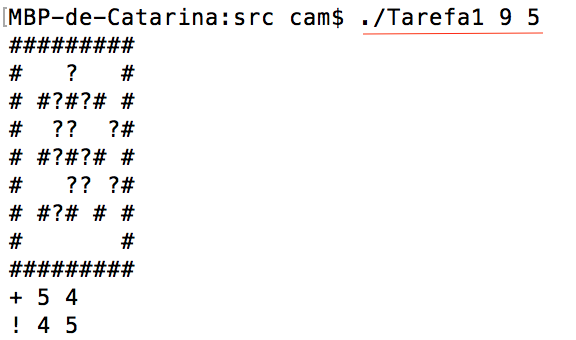
\includegraphics[scale=0.50]{tarefa1}
\caption{Exemplo de uma mapa de dimensão igual a 9, e semente igual a 5.}
\end{figure}

	\item Dando como parâmetros uma descrição do jogo, o identificador de um jogador\footnote{Cada 
  jogador é identificado por um dígito entre 0 e 3.} e um comando\footnote{Podem ser os caracteres \textbf{‘U’}
  (ir para cima), \textbf{‘D’} (ir para baixo), \textbf{‘L’} (ir para a esquerda), \textbf{‘R’} 
  (ir para a direita) e \textbf{‘B’} (colocar uma bomba).}, determinou-se o \underline{efeito desse comando no 
  estado de jogo.}
  	Para tal, adiciona-se linhas à descrição do estado de jogo; No caso das bombas, são identificadas pelo
  	caracter '*', sendo listada depois a sua posição, qual o jogador que a colocou, qual o seu raio
  	de ação, e quantos instantes de tempo que faltam para explodir; Os jogadores são identificados pelo
  	seu dígito, sendo listada depois a sua posição e os power ups que entretanto aculumou. (Tarefa 2);
	\item Dada uma descrição do jogo, foi necessário criar um mecanismo que permita poupar caracteres. 
	É necessário implementar um mecanismo no qual se \underline{comprima} o jogo e, após a descompressão, se obtenha o 
	estado de jogo incial. Um exemplo da utilização deste mecanismo é ao colocar o jogo em pausa: existem 
	certos caracteres que são sempre fixos ao longo do jogo. Para tal, utilizamos a função \textsf{'encode'}. 
	Ao retomar o jogo, é utilizada a função \textsf{'decode'}. Como se observa, para um estado de jogo \textit{m}, é necessário que \textbf{'decode (encode m) = m'}. (Tarefa 3).
\end{enumerate}

Nesta 2ª, e última, fase, é proposto que se conclua o projeto, de modo a 
produzirmos então o nosso primeiro programa em Haskell: \texttt{o jogo Bomberman completo}. 
Para tal, fica implícito que se deve:

\begin{enumerate}
	\item Determinar o \underline{efeito da passagem de um instante de tempo} no estado de jogo, 
	tendo em especial consideração a explosão de bombas, e o efeito espiral\footnote{No final de cada jogo,
  o mapa começa a fechar-se com blocos de pedra num efeito de espiral que começa na posição 1 1.} (Tarefa 4);
	\item Construir a \underline{interface gráfica} do jogo utilizando a biblioteca Gloss, onde 
	se procura estimular o nosso lado mais criativo, de modo a produzir um jogo com um aspecto 
	apelativo, e, jogável (Tarefa 5);
	\item Elaboração de um \underline{bot que jogue Bomberman automaticamente}, tendo em conta que se 
	trata de um jogo \textit{multiplayer}, e, assim, o bot poderá ser utilizado quando menos de 4 humanos 
	quiserem jogar. Desta forma, procura-se que o bot tenha um certo grau de inteligência, de modo a 
	tornar o jogo mais aliciante para todos os adversários (Tarefa 6).
\end{enumerate}

Neste caso, a Secção~\ref{sec:problema} descreve o problema a resolver, devidamente 
repartida nas Secções~\ref{sec:problemaTarefa4},~\ref{sec:problemaTarefa5} e~\ref{sec:problemaTarefa6}, 
para uma descrição mais detalhada de cada um dos 3 principais problemas a resolver. Por outro 
lado, a Secção~\ref{sec:solucao} apresenta e discute a solução por nós implementada, mais uma 
vez dividida nas Secções~\ref{sec:solucaoTarefa4},~\ref{sec:solucaoTarefa5} e~\ref{sec:solucaoTarefa6}. 
O relatório termina com conclusões na Secção~\ref{sec:conclusao}, onde é também apresentada
uma análise crítica dos resultados obtidos.

\section{Descrição do Problema}
\label{sec:problema}

De forma a desenvolver a 2.ª fase do projeto de Laboratórios de 
Informática I, e como anteriormente explicado, nesta etapa tem que se 
resolver as últimas 3 tarefas (Tarefas 4, 5 e 6), para assim se obter o 
jogo inteiramente operacional.

\subsection{Tarefa 4}
\label{sec:problemaTarefa4}

A primeira tarefa desta fase (\textbf{Tarefa 4}), consiste no efeito da passagem
do tempo. A passagem do tempo tem como consequência principal a explosão 
de bombas. Cada bomba demora 10 instantes de tempo a explodir. Quando explode,
lança chamas com dimensão igual ao raio\footnote{O raio de acção de
  uma bomba é determinado pelo número de power ups flame que o jogador possuía quando plantou a bomba.} nas
quatro direções principais (norte, sul, leste e oeste).

Deste modo, para a efetiva explosão das mesmas deve-se ter em consideração que:

\begin{itemize} 
	\item Numa determinada direção, quando as chamas atingem um bloco do
	tipo \textbf{pedra}, não o destroem, e a sua passagem é bloqueada pelos mesmos;
	\item A passagem das chamas também é bloqueada pelos \textbf{tijolos} e \textbf{power ups} (destapados),
	sendo que, nestes casos, tanto os tijolos, como os power ups, são destruídos, e, 
	consequentemente, eliminados da representação do jogo;
	\item Se as chamas atingirem outra \textbf{bomba} o temporizador dessa bomba passa para 1,
	de forma a forçar a sua explosão no próximo instante de tempo;
	\item Quando encontra um \textbf{jogador}, esse jogador tem que ser automaticamente eliminado do jogo.
\end{itemize}

É também importante ter em atenção que pode existir mais do que um jogador, ou até mesmo 
vários jogadores e uma bomba na mesma célula, e que várias bombas podem explodir em simultâneo 
e atingir coordenadas em comum.

Em consequência, se nenhuma bomba explodir no próximo estado de tempo, simplesmente
passou 1 instante de tempo, e os jogadores continuaram a mover-se como bem entenderam.

O outro aspecto fulcral desta tarefa é o \textbf{efeito espiral}. Sendo \textit{n} a dimensão do mapa,
quando faltarem ${(n-2)^2}$ instantes de tempo para o jogo terminar, o mapa começa 
a fechar-se com blocos de pedra num efeito espiral. Em cada instante de tempo cai 
um bloco de pedra que elimina tudo o que estiver na respetiva posição, sejam jogadores, 
tijolos, power ups destapados ou bombas.

Assim, deve-se implementar a função \textsf{'avanca'}, que tem como parâmetros o estado atual
do jogo e o número de instantes de tempo que faltam para o jogo terminar, e que devolverá
como resposta o novo estado de jogo, devidamente atualizado.

\subsection{Tarefa 5}
\label{sec:problemaTarefa5}

A segunda tarefa da 2ª fase do projeto tem como objetivo implementar o jogo completo usando a biblioteca \emph{Gloss}.

Para esta Tarefa foram necessárias as funções \textsf{'mapa'}, \textsf{'move'} e \textsf{'avanca'}, implementadas nas 
tarefas 1, 2 e 4, respetivamente.

É necessário começar por uma visualização gráfica simples, ou seja, utilizando um mapa com dimensões e sementes fixas. 

Um outro tópico desta Tarefa que é necessário para o jogo fluir é a decisão das teclas usadas por cada jogador 
para que o jogo avance. Foi feita a função \textsf{'reageEvento'} para que algo aconteça no jogo a partir do 
momento em que o jogador carregue numa tecla. Foi utilizada como auxílio a função \textsf{'move'} implementada 
anteriormente.

Finalmente, é necessário implementar o jogo nas funções \textsf{'estadoInicial'} e \textsf{'desenhaEstado'}.
O tempo do jogo será escolhido pelo próprio computador a partir da função \textsf{'time'} e consequentemente uma função
que fará o jogo avançar recorrendo à função \textsf{'avanca'}.

Depois de todas as funções estarem implementadas na função abrangente \textsf{'main'} o jogo estará pronto 
para ser testado e jogado!

\subsection{Tarefa 6}
\label{sec:problemaTarefa6}

Na terceira, e última, tarefa da 2.ª fase do projeto (\textbf{Tarefa 6}) o objetivo
será implementar um estratégia de combate, isto é, elaborar um \emph{bot} que jogue 
Bomberman automaticamente. 

Para o seu desenvolvimento, tem que se ter em consideração que o bot irá receber 
como parâmetros o número de instantes que faltam para o jogo terminar, e a descrição 
atual do jogo (sendo que o bot, tal como os comuns jogadores, não tem acesso às coordenadas 
dos power ups que ainda se encontram escondidos atrás de tijolos).

Como já mencionado, é essencial que o bot tenha um generoso grau de \emph{inteligência}. Tendo
em conta que existem somente duas formas de um jogador ser eliminado do jogo, sendo elas 
ser atingido pelas chamas de uma bomba, ou em consequência do efeito espiral, na nossa opinião 
é primordial que o bot saiba fugir excecionalmente das bombas, e que, na parte final do 
jogo, a sua estratégia se encontre alterada de modo a não cair nenhuma pedra em cima dele.

O objetivo é que o bot saiba também procurar os tijolos e os jogadores no mapa, 
para assim, consequentemente, os destruir. Deverá também procurar os power ups destapados, 
para conseguir evoluir a quantidade e o raio de destruição das suas bombas. 

Deve-se então implementar a função \textsf{'bot'}, que dará como resposta o comando que o 
bot deverá executar (\emph{Just ‘L’}, \emph{Just ‘R’}, \emph{Just ‘D’}, \emph{Just ‘U’} ou \emph{Just ‘B’}), 
ou ainda \textit{Nothing} se não for conveniente utilizar algum comando.

\section{Concepção da Solução}
\label{sec:solucao}

Para o desenvolvimento deste projeto teve-se em consideração
vários aspetos, e ao longo da sua elaboração foram múltiplas as adversidades 
que surgiram. Em seguida seguem-se as estruturas e procedimentos que adotados 
para a resolução do \emph{problema}.

\subsection{Estruturas de Dados}

Para a solução implementada, a estrutura de dados mais recorrente foi a \emph{type synonyms}. 
Se se tivesse utilizado sempre uma estrutura do tipo \emph{record syntax}, 
com certeza que se tinha tido muito menos trabalho na elaboração de todas as funções, 
uma vez que se teve que estar constantemente a “desdobrar” o estado de jogo. Porém, 
a estrutura de dados utilizada também contribuiu para um código mais \textrm{intuitivo}, 
e de melhor \textrm{compreensão}.

Deste modo, os \emph{types} que foram considerados mais benéficos para o problema 
em questão foram os seguintes: 

\begin{figure}[H]
\centering 
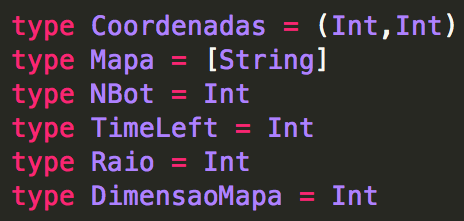
\includegraphics[scale=0.50]{types}
\caption{Types.}
\end{figure}

\subsection{Implementação}

Como forma de atingir os objetivos propostos, seguidamente apresentam-se, 
de forma pormenorizada, as \textbf{soluções} propostas, e implementadas, para cada 
uma das 3 tarefas do \textbf{problema}.

\subsubsection{Tarefa 4}
\label{sec:solucaoTarefa4}

Para a efetiva resolução desta tarefa, começou-se por dividir-la em dois passos:

\begin{enumerate} 
	\item \underline{Explosão de bombas} (ou simples passagem do tempo 
	quando nenhuma bomba explode no próximo instante de tempo);
	\item \underline{Efeito Espiral}.
\end{enumerate}

No primeiro passo, começou-se por descobrir quais as \textbf{coordenadas} e os respetivos 
\textbf{raios} das bombas que iam explodir no próximo instante de tempo.

De seguida, fez-se funções que dessem como resposta o que estava \emph{concretamente} 
nas coordenadas abaixo, acima, à esquerda e à direita das coordenadas da bomba que vai 
explodir (tendo em conta o raio da mesma). As alternativas possíveis são as seguintes:
\begin{enumerate} 
	\item Pedra;
	\item Tijolo;
	\item Power up; 
	\item Bomba;
	\item Jogador;
	\item Nada.
\end{enumerate}

Deste modo, para a resolução desta tarefa, foi crucial a elaboração de \emph{6 funções}, 
que são os \hypertarget{6funções}{\underline{mapas de resposta ao problema}}. Todas estas funções têm como parâmetros 
o estado atual do jogo e um par de coordenadas (x,y) afetadas.

\begin{itemize}
	\item A primeira função, denominada por {\large\textbf{“novoMapaSE”}} retira 1 instante de 
	tempo a todas as bombas presentes no mapa (após as que tinham que explodir efetivamente
	explodirem).
	\item A segunda função, designada por {\large\textbf{“novomapaComInst1”}}, dá como resultado o
	mapa com a bomba que foi atingida por outra bomba que explodiu, com os instantes de
	tempo devidamente alterados (neste caso com instantes = 2, porque a função mencionada 
	anteriormente \emph{(“novoMapaSE”)} vai retirar mais 1 instante de tempo).
	\item A terceira função, denominada {\large\textbf{“novomapaSemJog”}} dá como resposta o novo
	mapa atualizado, sem as linhas relativas aos jogadores que acabaram de perder.
	\item A quarta função, com o nome de {\large\textbf{“novomapaSemPU”}}, devolve a nova descrição
	do jogo, sem a linha referente ao power up atingido. 
	\item A quinta função, denominada {\large\textbf{“novomapaSemPI”}} dá como resposta o mapa sem 
	o tijolo que foi atingido por chamas.
	\item E, por fim, a função {\large\textbf{“novomapaSemBombaExpl”}} que dá como resultado o 
	mapa sem a linha relativa à bomba que estava nas coordenadas passadas como parâmetros.
\end{itemize}


Assim sendo, tem-se todos os alicerces necessários para a conclusão desta parte da tarefa, 
bastava somente interliga-los. Com recurso a 4 simples funções, nomeadamente \emph{\textbf{"oqueaconteceD"}},
\emph{\textbf{"oqueaconteceU"}}, \emph{\textbf{oqueaconteceL"}} e \emph{\textbf{"oqueaconteceR"}}, 
faz-se "explodir" o que estava nas coordenadas para baixo, cima, esquerda e à direita da bomba, respetivamente.

Na Figura~\ref{img:oqueaconteceD} encontra-se representada a função \emph{"oqueaconteceD"}, a primeira das 4 funções
do processo efetivo de explosão. Assim, consegue-se notar que sabendo o que está \emph{concretamente} nas 
coordenadas afetadas, e com recurso às 6 funções anteriormente expostas, o processo de explosão das bombas 
encontra-se concluído. 

\begin{figure}[H]
\centering 
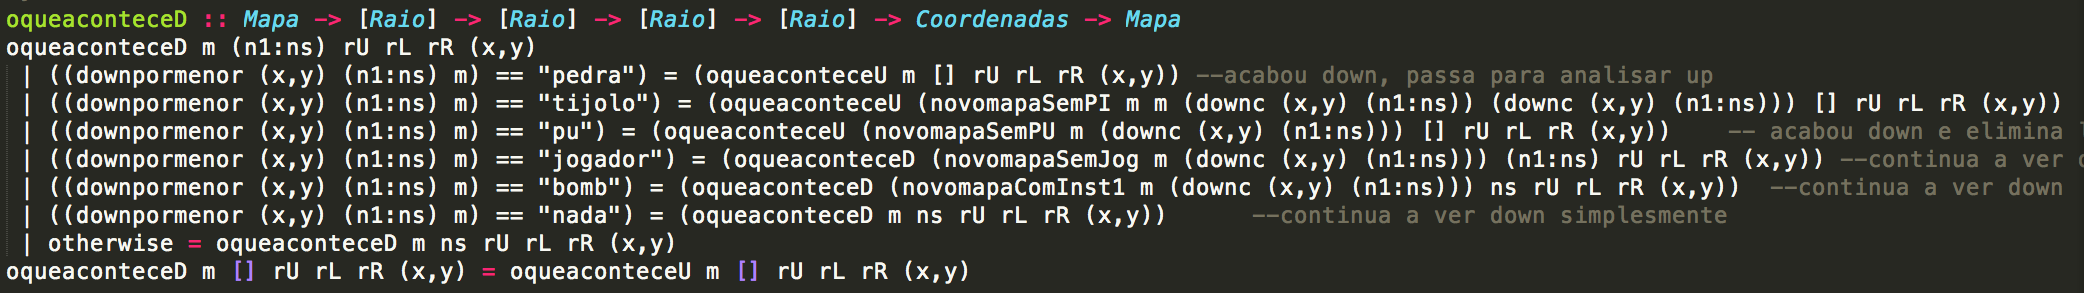
\includegraphics[scale=0.40]{oqueaconteceD}
\caption{Função que explode o que está nas coordenadas abaixo da bomba.}
\label{img:oqueaconteceD}
\end{figure}

Porém, mais tarde, apercebemo-nos que as bombas explodiam corretamente o que estava ao seu redor, 
mas não eliminavam o que estava nas suas \textbf{próprias coordenadas} (nomeadamente, possíveis jogadores). 
Para a resolução deste problema, bastou elaborar uma função que analisa o próprio pormenor da bomba, 
e adicioná-la no princípio do processo, como se pode ver na Figura~\ref{img:verificaCaminho}.

\begin{figure}[H]
\centering 
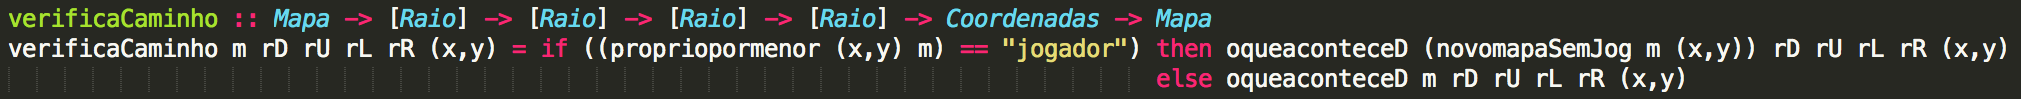
\includegraphics[scale=0.40]{verificaCaminho}
\caption{Função que verifica se tem algum jogador na coordenada da bomba, e prossegue o processo de explosão.}
\label{img:verificaCaminho}
\end{figure}

Posteriormente, com a ajuda dos testes, deparamo-nos com outro \emph{erro} importante. No jogo, 
as bombas estavam a explodir uma de cada vez, ao invés de todas ao mesmo tempo. Numa situação em 
que várias bombas explodem em simultâneo e atingem coordenadas em comum, a resposta obtida não era 
a esperada. Assim, fez-se uma pequena alteração de modo a solucionar este problema.

Em primeiro, fez-se uma função que dá como resposta as coordenadas que são afetadas pelas \textbf{chamas 
das bombas}, no próximo instante de tempo. Assim, se houvesse coordenadas repetidas nessa lista, 
significava que esse caso iria cair no atual problema. 

Com o recurso às funções com os \hyperlink{6funções}{mapas de resposta ao problema}, como já se tem 
as coordenadas afetadas pelas chamas, basta passar essas coordenadas como argumento nas outras 
funções, e, assim, elimina-se/altera-se o necessário no estado do jogo.

Assim, tanto o método inicialmente adotado, como este novo método continuarão a ser utilizados.
\begin{enumerate} 
	\item \textbf{"prossegue"}, é a função corresponde ao meio inicial;
	\item \textbf{"variasBombasExplodem"}, é a função relativa ao novo meio.
\end{enumerate}

Através da função apresentada na Figura~\ref{img:analisa} consegue-se encaminhar 
corretamente o problema exposto, uma vez que a função \emph{"coincide"} irá dizer se bombas diferentes 
atingem coordenadas em comum. 

\begin{figure}[H]
\centering 
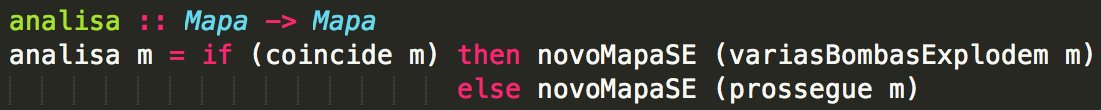
\includegraphics[scale=0.40]{analisa}
\caption{Função que faz explodir todas as bombas corretamente.}
\label{img:analisa}
\end{figure}

Deste modo, para concluir efetivamente este primeiro passo da tarefa, 
ligou-se todas estas funções da seguinte forma:

\begin{enumerate} 
	\item Se \emph{alguma} bomba explodir, então todo o processo é analisado pela função referida na 
	figura~\ref{img:analisa}.
	\item Se \emph{nenhuma} bomba explodir, então retira-se simplesmente 1 instante de tempo a todas
	as bombas plantadas no mapa.
\end{enumerate}

\begin{figure}[H]
\centering 
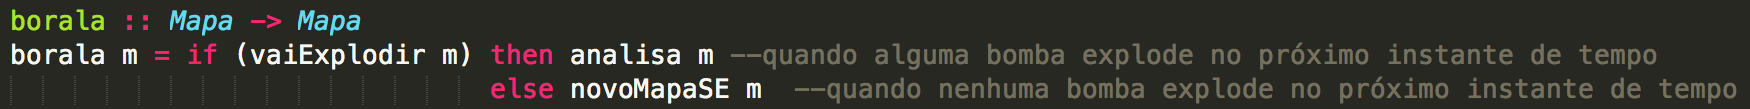
\includegraphics[scale=0.40]{borala}
\caption{Função que dá como resultado o mapa quando há bombas a explodir, ou quando nenhuma bomba explode.}
\label{img:borala}
\end{figure}

No segundo passo, para a implementação do \underline{efeito espiral} que surge no 
final do jogo, concluiu-se que caso se soubessem as \textbf{coordenadas
em que a pedra seguinte iria cair}, com base nas funções já definidas, 
teria-se todo o problema resolvido.

Deste modo, começou-se por tentar detetar um \emph{padrão} na ordem das coordenadas 
(horizontais e verticais) pelas quais as pedras caiem. Por exemplo, num mapa de 
dimensão 9 a ordem é a seguinte:

\begin{table}[h]
\centering
\begin{tabular}[c]{ccccccc}
(1,1) & (2,1) & (3,1) & (4,1) & (5,1) & (6,1) & (7,1) \\
(7,2) & (7,3) & (7,4) & (7,5) & (7,6) & (7,7) & (6,7) \\
(5,7) & (4,7) & (3,7) & (2,7) & (1,7) & (1,6) & (1,5) \\
(1,4) & (1,3) & (1,2) & (2,2) & (3,2) & (4,2) & (5,2) \\ 
(6,2) & (6,3) & (6,4) & (6,5) & (6,6) & (5,6) & (4,6) \\
(3,6) & (2,6) & (2,5) & (2,4) & (2,3) & (3,3) & (4,3) \\
(5,3) & (5,4) & (5,5) & (4,5) & (3,5) & (3,4) & (4,4)
 \end{tabular}
\caption{Ordem do Efeito Espiral num mapa de dimensão 9} 
\label{table:espiral}
\end{table}

Analisando separadamente as coordenadas horizontais (\textbf{X}) e verticais (\textbf{Y}), tem-se:

\begin{table}[!htb] 
\begin{minipage}[b]{0.40\linewidth}
\begin{tabular}[c]{cll}
X: & (1,2,3,4,5,6,7) & (7,7,7,7,7,7) \\ \
  & (6,5,4,3,2,1) & (1,1,1,1,1) \\
  & (2,3,4,5,6) & (6,6,6,6) \\
  & (5,4,3,2) & (2,2,2) \\ 
  & (3,4,5) & (5,5) \\
  & (4,3) & (3) \\
  & (4)
 \end{tabular}
\caption{Ordem das coordenadas X.}
\label{table:espiralx}
\end{minipage} \hfill 
\begin{minipage}[b]{0.40\linewidth} 
\begin{tabular}[c]{cll}
 Y: & (1,1,1,1,1,1,1) & (2,3,4,5,6,7) \\
  & (7,7,7,7,7,7) & (6,5,4,3,2) \\
  & (2,2,2,2,2) & (3,4,5,6) \\
  & (6,6,6,6) & (5,4,3) \\ 
  & (3,3,3) & (4,5) \\
  & (5,5) & (4) \\
  & (4) 
 \end{tabular}
\caption{Ordem das coordenadas Y.}
\label{table:espiraly}
\end{minipage}
\end{table}

Assim, com recurso a simples funções como \textit{replicate}, \textit{reverse} e 
\textit{list ranges} conseguiu-se construir as coordenadas X e as coordenadas Y 
pela ordem em que as pedras caiem. Através da função \textit{zip} agrupou-se essas 
coordenadas X e Y, e obtive-se assim a função que dá os pares das coordenadas 
pela devida ordem, tal como na Tabela~\ref{table:espiral}.

Em seguida, fez-se uma função que descobria qual era a coordenada que a 
próxima pedra ia atingir. Para isso, fez-se uma função que inicialmente reverte a lista, 
e, assim, basta “pegar” na coordenada que está na posição igual ao número de 
instantes que faltam para o jogo terminar.

Deste modo, para \textbf{colocar a pedra na representação do jogo}, como já se sabem as 
coordenadas (x,y) em que a pedra cai, com a ajuda da função (!!) (já definida na 
prelude do Haskell) basta ir à linha y, e posição x, e substituir o que lá estiver por uma
pedra (\#).

Assim, falta apenas averiguar o que estava na coordenada em que a pedra caiu, podendo ser: 

\begin{enumerate} 
	\item \textbf{Uma bomba}, e em caso afirmativo, com recurso à 
	função \emph{“novomapaSemBombaExpl”} eliminou-se essa bomba da representação do jogo;
	\item \textbf{Power ups destapados}, e em caso afirmativo, com a ajuda da função 
	\emph{“novomapaSemPU”}, excluiu-se o power up da representação do jogo;
	\item \textbf{Jogadores}, e neste caso, com recurso à função \emph{“novomapaSemJog”} 
	removeu-se todos os jogadores que pudessem estar nessas coordenadas.
\end{enumerate}

Para assim finalizar a Tarefa 4, com recurso à função da Figura~\ref{img:tempo} (que, consoante o tempo 
que falta para o jogo acabar, insere (ou não) o efeito de espiral no jogo), e, à função pedida no
enunciado, a função \textbf{"avanca"}, representada na Figura~\ref{img:avanca}, 
obteve-se então a \textbf{Tarefa 4 concluída}.

\begin{figure}[H]
\centering 
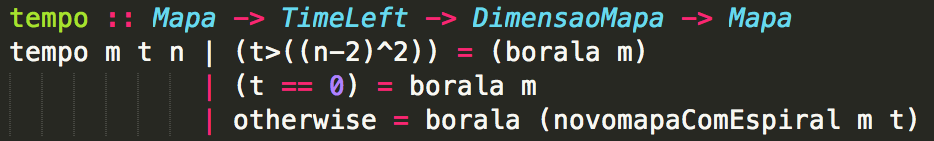
\includegraphics[scale=0.40]{tempo}
\caption{Função que devolve o mapa com o novo instante de tempo.}
\label{img:tempo}
\end{figure}

\begin{figure}[H]
\centering 
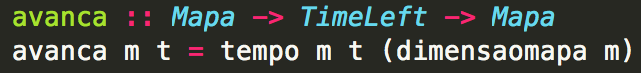
\includegraphics[scale=0.40]{avanca}
\caption{Função que dá resposta à Tarefa 4.}
\label{img:avanca}
\end{figure}

\subsubsection{Tarefa 5}
\label{sec:solucaoTarefa5}

Para esta tarefa, existem várias soluções visto que, o mapa tanto poderá ser de dimensão 
e sementes fixas determinadas pelos criadores, como poderá ser à escolha do jogador.

O primeiro passo para a realização desta tarefa, foi "partir" um mapa com informação 
implementada na Tarefa 1 da 1ª fase, 
uma nova forma para a sua observação que, será de mais fácil observação. A partir deste 
raciocínio, foi possível criar 
um novo \emph{Estado} de jogo, que conterá a mesma informação de um mapa inicial do 
tipo \textsf{[String]} para o tipo
\textsf{EstadoV}. Mais tarde foi necessário ainda implemetar o tipo \textsf{Estado} com 
informação relativa ao mapa, às imagens e ao tempo de jogo. 

É necessário reforçar que as únicas imagens suportadas foram em tipo \emph{Bitmap}. 

\subsubsection{Tarefa 6}
\label{sec:solucaoTarefa6}

Para a implementação de uma estratégia de combate, o primeiro passo foi a elaboração
de uma função que excluísse as direções para onde o bot não pode ir, uma vez que este não se 
pode mover para células onde haja \textbf{tijolos} ou \textbf{pedras}. Para este caso em 
específico, existem 15 diferentes possibilidades.

\begin{figure}[H]
\centering 
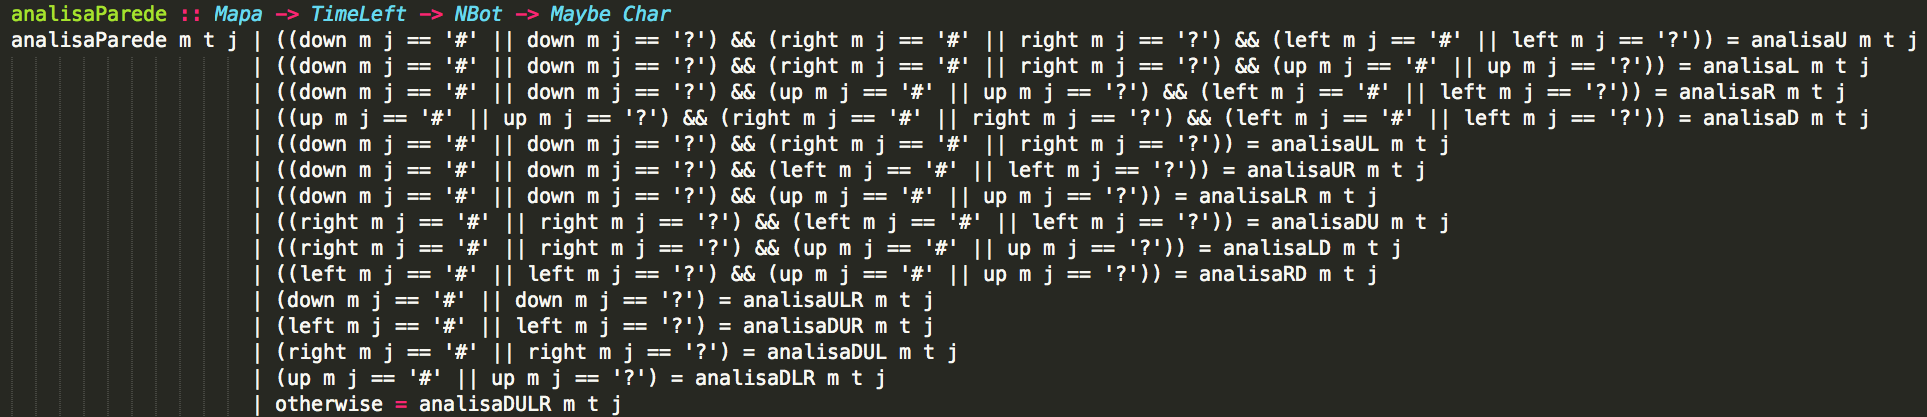
\includegraphics[scale=0.50]{analisaParede}
\caption{Função que ajuda na decisão do comando do bot, consoante as direções que ele pode efetivamente ir.}
\end{figure}

Assim, analisando somente as coordenadas "disponíveis", o segundo passo consistiu em
averiguar se o \textbf{bot estava em perigo}\footnote{O bot encontra-se em perigo se as 
  chamas de alguma das bombas plantadas atingem essas coordenadas.} se ficasse quieto, 
ou se fosse para alguma das coordenadas possíveis. Deste modo, em caso de não haver dúvidas 
relativamente a qual direção escolher, ele opta por essa (por exemplo, se o bot só tem disponíveis 
as direções \emph{up} e \emph{down}, e se encontra em perigo na coordenada 
atual e também estaria em perigo se fosse para cima, a opção será ir para baixo). Se porventura está 
em perigo em qualquer das alternativas, com recurso às funções \emph{"fugir"}, o bot consegue analisar 
em média cerca de \underline{1/4 do mapa} (em seu redor), de modo a conseguir optar corretamente pela 
direção que o ajudará a "ficar em segurança" mais rapidamente. Na Figura~\ref{img:analisaLR}, nas 
primeiras 4 guardas da função consegue-se verificar o procedimento adotado.

Em seguida, se após excluídas as coordenadas pelas quais o bot não pode optar (uma vez que ficaria em 
perigo), ainda restarem 2 ou mais opções possíveis\footnote{No total existem 5 opções possíveis, sendo elas
  ir para baixo, ir para cima, esquerda, direita, ou manter-se na mesma célula.}, a decisão é encaminhada
para outra função \emph{("tempoATerminar")}, que faz o seguinte:

\begin{itemize}
	\item Analisa o tempo que falta para o jogo terminar, e se faltarem \textbf{15 ou menos} instantes
	de tempo, o processo é analisado na função \emph{"encurralado"}, que averigua se
	está algum tijolo no sítio para onde o bot pretende ir, e, em caso afirmativo, planta uma bomba, caso
	contrário, o processo é analisado na função \emph{"fugirEspiral"}, que, como o nome indica, ajuda o bot 
	a fugir do efeito espiral;
	\item Se faltarem \textbf{mais de 15} instantes de tempo para a espiral começar, a decisão do bot
	é encaminhada para a função \emph{"plantaBombas"}.
\end{itemize}

Para \underline{fugir da espiral}, o bot opta pela direção em que a distância até à célula onde cai a
última pedra do mapa é menor.

Na Figura~\ref{img:analisaLR}, nas últimas 3 guardas da função, e na Figura~\ref{img:tempoATerminarLR}
consegue-se verificar o sucedido.

\begin{figure}[H]
\centering 
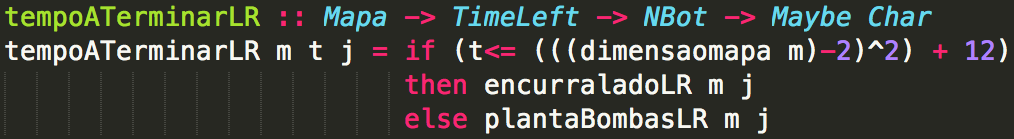
\includegraphics[scale=0.50]{tempoATerminarLR}
\caption{Averigua se o tempo para o jogo terminar está quase a acabar.}
\label{img:tempoATerminarLR}
\end{figure}

No caso da função que \underline{planta bombas}, se estiver algum tijolo ou jogador em torno do bot, 
ele planta uma bomba. Caso contrário, o processo segue a seguinte sequência:

\begin{enumerate} 
	\item Procura \textbf{power ups} no mapa num raio de 3 células (somente nas direções 
	possíveis ao movimento);
	\item Procura \textbf{tijolos} no mapa, também num raio de 3 células para as direções 
	possíveis ao movimento;
	\item Procura \textbf{jogadores}, num raio de 3 células para as direções possíveis, e, 
	se não encontrar nenhum, vai para uma coordenada "aleatória".
\end{enumerate}

Na Figura~\ref{img:analisaLR}, na 5ª guarda, nota-se um caso diferente, em que o bot não 
pode ficar na coordenada em que se encontra, e, deste modo, não poderá plantar uma bomba visto
que isso teria como consequência manter-se na mesma coordenada. Assim, o processo de decisão
decorrerá somente através da enumeração anterior, começando assim analisando os power ups em 
seu redor.

\begin{figure}[H]
\centering 
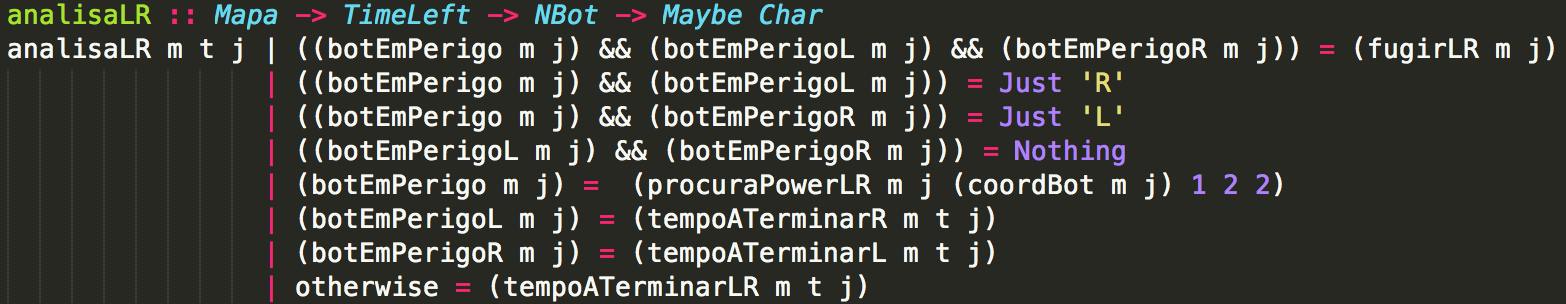
\includegraphics[scale=0.50]{analisaLR}
\caption{Decide o que o bot deve fazer, tendo em conta que só pode ir para a esquerda ou direta.}
\label{img:analisaLR}
\end{figure}

Tendo em consideração que quando era necessário recorrer à coordenada "aleatória", a opção foi
sempre \emph{"down"} ou \emph{"right"} (para não originar ciclos), no caso do bot estar 
indeciso entre \emph{"up"} e \emph{"left"}, o bot vai dar como resposta \emph{Nothing}.
Ou, se não for possível, irá então para \emph{"up"} ou \emph{"left"}.

\subsection{Testes}

De modo a produzir um jogo sem \emph{bugs}, e, assim, o mais \textbf{completo} possível,
a elaboração de testes foi essencial, uma vez que ajudaram bastante na deteção de eventuais
erros ou pormenores que não tinham sido corretamente explorados.

Em seguida, seguem-se alguns dos exemplos realizados:

\begin{figure}[H]
\centering 
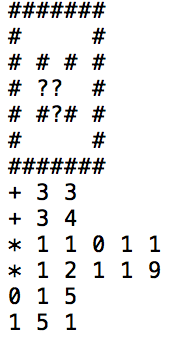
\includegraphics[scale=0.40]{exemplo24}
\caption{{\small Exemplo que procura testar quando uma bomba explode, e as suas chamas atingem outra bomba.}}
\end{figure}

\begin{figure}[H]
\centering 
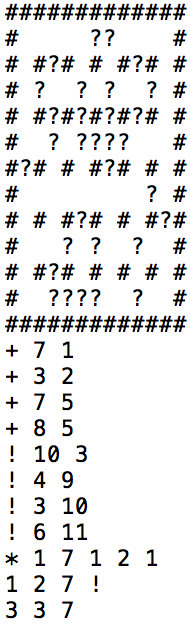
\includegraphics[scale=0.40]{exemplo25}
\caption{{\small Exemplo que procura testar a hipótese de 2 jogadores perderem ao mesmo tempo.}}
\end{figure}

\begin{figure}[H]
\centering 
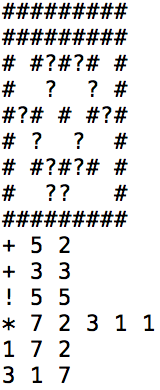
\includegraphics[scale=0.40]{exemplo28}
\caption{{\small Exemplo que procura testar o facto de uma pedra cair numa célula que tenha 
simultaneamente jogadores e bombas.}}
\end{figure}

\begin{figure}[H]
\centering 
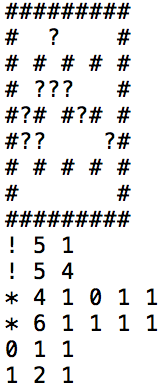
\includegraphics[scale=0.40]{exemplo38}
\caption{{\small Exemplo que procura testar o caso de diferentes bombas atingirem as mesmas
coordenadas.}}
\end{figure}

\section{Conclusões}
\label{sec:conclusao}

Nesta trabalho abordámos o desenvolvimento do projeto do jogo \textbf{Bomberman},
que se encontrava dividido em 6 tarefas, onde 3 delas já tinham sido 
anteriormente resolvidas. Nesta 2ªfase, e nestas últimas 3 tarefas do projeto, 
só cumprimos alguns dos objetivos uma vez que a Tarefa 5 não se encontra operacional. 
Em seguida, apresenta-se uma análise crítica de cada uma das tarefas desta fase.

Na primeira tarefa desta fase \underline{(Tarefa 4)}, tendo em conta todos os testes 
que se efetuou, o resultado foi o pretendido, dado que o efeito da passagem do tempo se
encontra corretamente definido no nosso jogo.

Na segunda tarefa desta fase \underline{(Tarefa 5)}, foi utilizado apenas um mapa de dimensão 
13 e semente 2 sendo, por isso, um mapa sempre fixo. Os resultados para esta tarefa não foram os 
pretendidos, visto que, apesar da tarefa compilar, não é possível realizar o efeito dos comandos. 

Na última tarefa \underline{(Tarefa 6)}, consideramos que o bot tem inteligência,
visto que sabe fugir das chamas das bombas, procura jogadores e tijolos, 
planta bombas oportunamente, e nos instantes finais, foge da espiral. Porém, o bot
poderia ser ainda melhor, por exemplo se ao invés de só conseguir procurar jogadores
e tijolos num raio de 3 coordenadas nas direções favoravéis ao movimento, conseguisse 
abranger todo o mapa (tal não foi possível porque desse modo demoraria demasiado tempo a calcular a jogada).

Este projeto foi muito importante para o aprofundamento dos nossos conhecimentos
relativamente à linguagem de programação funcional \emph{Haskell}. Todas as tarefas
realizadas contribuiram bastante para a prática desta linguagem. Além disso, o 
presente relatório contribuiu para a prática de utilização de \LaTeX{}.

\end{document}